\documentclass[12pt, openany]{report}
\usepackage[utf8]{inputenc}
\usepackage[T1]{fontenc}
\usepackage[a4paper,left=2cm,right=2cm,top=2cm,bottom=2cm]{geometry}
\usepackage[frenchb]{babel}
\usepackage{libertine}
\usepackage[pdftex]{graphicx}

\setlength{\parindent}{0cm}
\setlength{\parskip}{1ex plus 0.5ex minus 0.2ex}
\newcommand{\hsp}{\hspace{20pt}}
\newcommand{\HRule}{\rule{\linewidth}{0.5mm}}

\begin{document}

\begin{titlepage}
  \begin{sffamily}
  \begin{center}

    % Upper part of the page. The '~' is needed because \\
    % only works if a paragraph has started.
    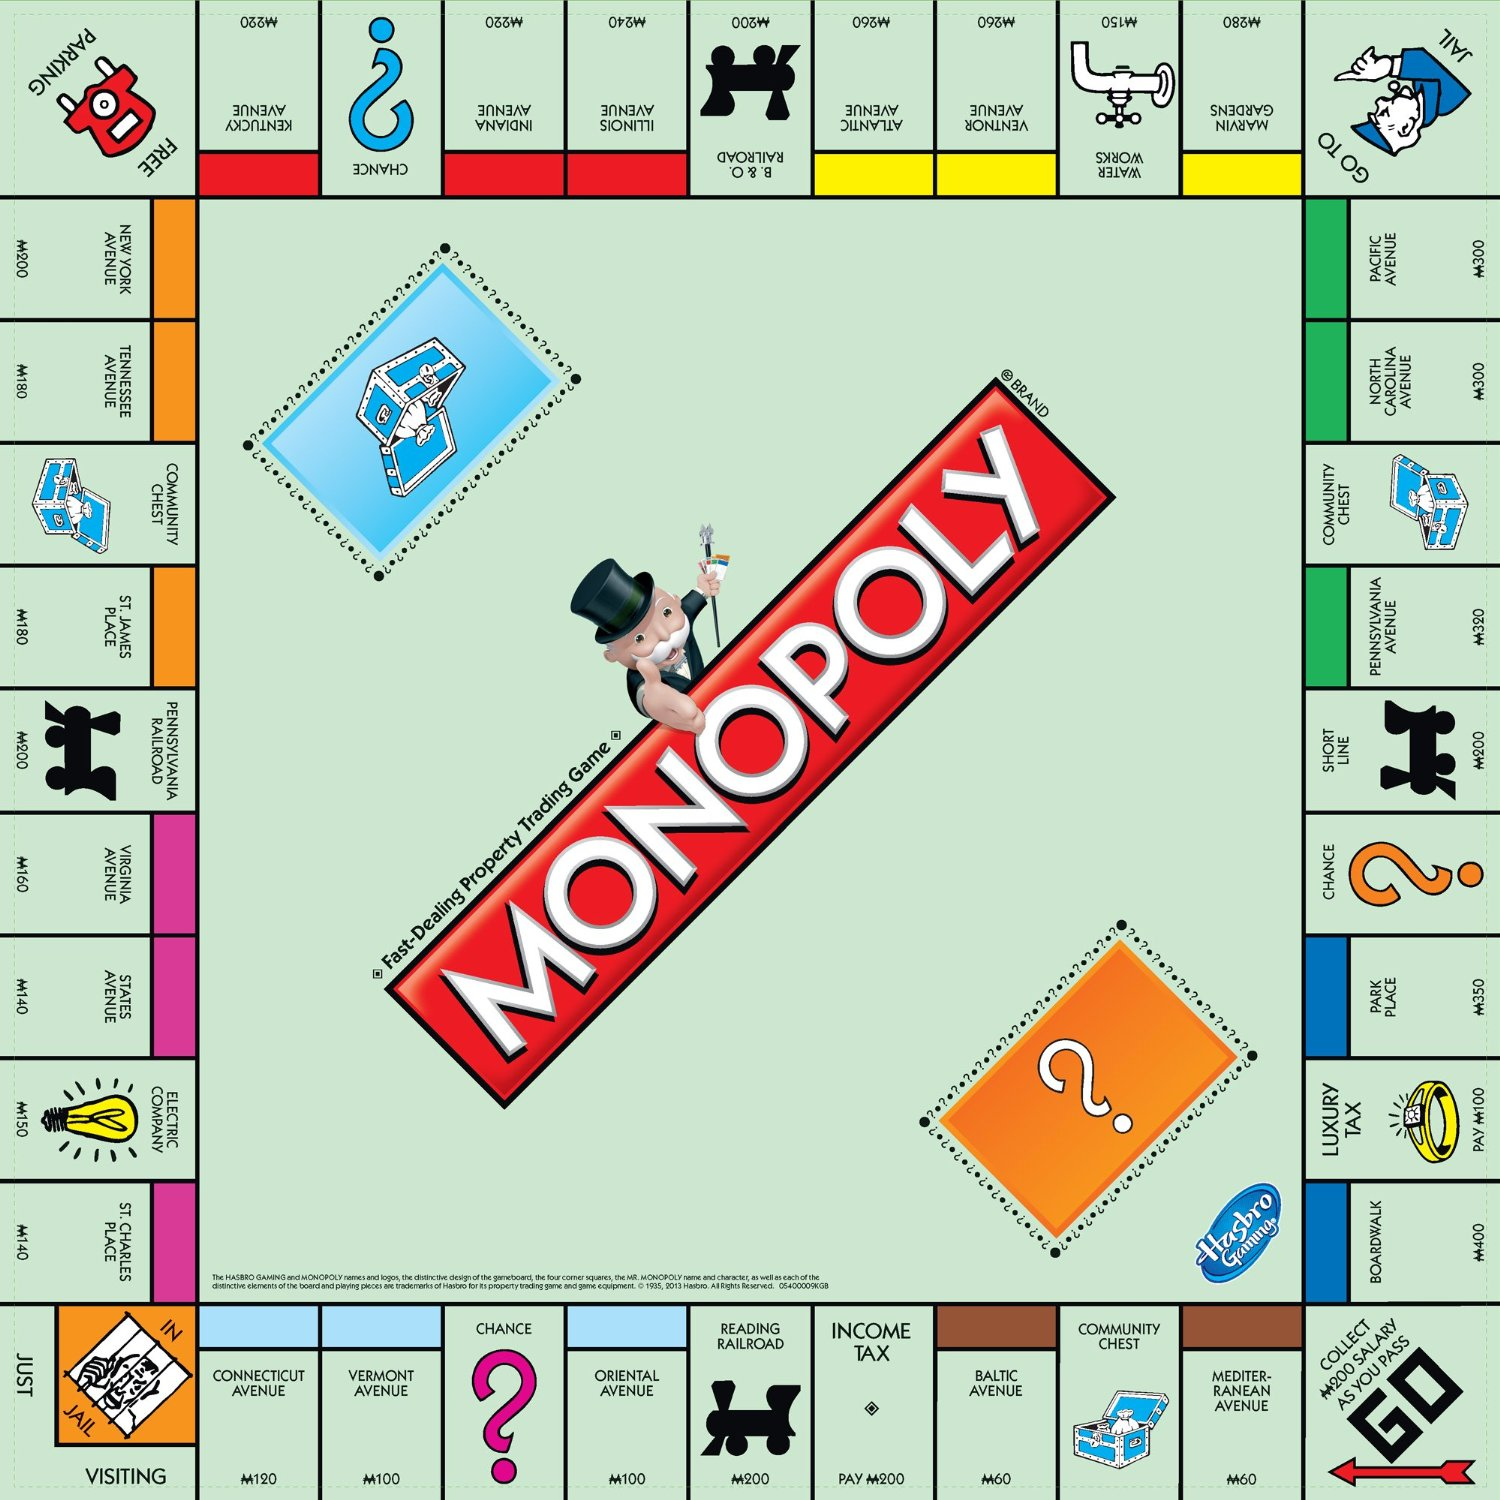
\includegraphics[scale=0.1]{monop.jpg}~\\[1.5cm]

    \textsc{\LARGE Faculté Jean Perrin, Lens}\\[2cm]

    \textsc{\Large Licence 3 Informatique}\\[1.5cm]

    % Title
    \HRule \\[0.4cm]
    { \huge \bfseries Rapport de projet, Monopoly\\[0.4cm] }

    \HRule \\[2cm]
    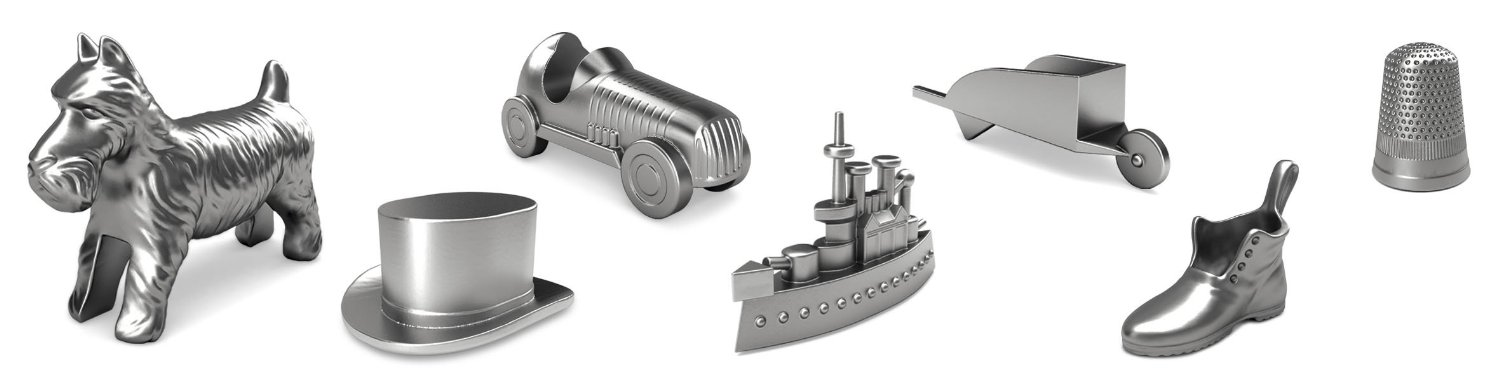
\includegraphics[scale=0.3]{pions.jpg}
    \\[2cm]

    % Author and supervisor
    \begin{minipage}{0.4\textwidth}
      \begin{flushleft} \large
        Nicolas \textsc{Serf}\\
        Promo 2017\\
      \end{flushleft}
    \end{minipage}
    \begin{minipage}{0.4\textwidth}
      \begin{flushright} \large
        \emph{Professeur :} M. \textsc{Piette}\\
      \end{flushright}
    \end{minipage}

    \vfill

    % Bottom of the page
    {\large 22 Mars 2017}

  \end{center}
  \end{sffamily}
\end{titlepage}

\newpage
\section{Résumé}
Le sujet de cette application est la réalisation du jeu monopoly comportant toutes les variantes les plus connues pour ce dernier. L'application se doit simple d'utilisation et ludique pour l'utilisateur. Les différentes variantes sont présentées dans le document de référence fournis par le professeur. La date limite de rendu de la première version du projet est le 21 mars 2017 avant 23h59. Nous avons cependant jusqu'au 30 avril 2017 pour finaliser notre application et fournir le rendu final.\\
Le réalisation de la première version du projet à rendre pour le 21 mars a été pour le moins compliqué au niveau gestion du temps car nous avions en même temps que ce monopoly:
\begin{itemize}
  \item Un projet de groupe en java : Tetris Attack 
  \item Un projet de TP par semaine en Java : (Othello en XML, bataille navale en reseau, Picross avec base de données, etc...)
  \item Un projet de PHP : Réalisation d'un site sur la bourse
  \item Un projet d'EE : Réaliser la simulation de création d'une entreprise en analysant tout les besoins
  \item Un projet de TE : Réaliser une présentation sur une innovation / invention d'un concept représentant l'internet des objets
\end{itemize}

\part{Le début du projet}
  \chapter{Création des documents}
    \section{Les documents fixes}
    Lorsque nous avons reçu le sujet du monopoly, j'ai tout de suite vu qu'il y avait beaucoup d'informations nécessaire à la création d'une partie de Monopoly. En effet, les différents cartes qui présentent le plateau de jeu et les différents cartes communautaires représentent des élèments fixes du jeu qui ne changent jamais. Ainsi, la première chose que jai réalisé est la mise en forme de ces informations dans un fichier XML pour pouvoir les charger facilement dans l'application Java. Ainsi, l'application se détache complétement de ces informations et n'a besoin que de les lire. Pareil pour les cartes chance et communautaire, les informations sur ces cartes ainsi que leurs descriptions sont présentes dans un fichier XML qui n'a plus qu'à être chargé pour construire les différentes cartes.\\\\
    Ces différents documents se trouvent dans /resources/files/. Ces documents sont sensé être immuable car ces données restent fixes quelque soit l'état de l'application.
    
    \section{Les documents de conception}
    Pour facilité le développement, je suis passé par une étude préalable d'un diagramme de classe pour représenter l'architecture de mon application. Cependant, me rendant compte qu'il allait falloir un peu d'essai avant d'aboutir à une version potable, j'ai commencé assez rapidement à faire des tests et à coder de petites choses. C'est finalement par la suite que j'en suis arrivé à un diagramme de classe qui me semblait correct compte tenu de mon architecture. Ce diagramme m'a permis durant la phase de développement de suivre une ligne de conduite et de ne pas m'éparpiller dans toutes les directions.\\\\
    Voici le diagramme de classe en question simplifié à son maximum. Le but est ici de simplement voir comment l'architecture MVC et mes classes se comportent et communiquent.\\\\
    \includegraphics[scale=0.4]{diagram.png}
  \chapter{Répartition des tâches}
    \section{Répartition des tâches du menu}
    Nous étions imposé de réaliser une partie menu pour une date donnée durant la première période de développement. J'ai ainsi décidé de lister les différents élèments devant être réalisé dans la partie menu et de les classer par ordre de priorité à réaliser. Ce classement s'est fait assez naturellement car certaines étapes nécessitent des précédentes.
    \begin{itemize}
      \item Réaliser la page principale du menu avec les différents boutons
      \item Linker les différents boutons pour envoyer vers les différents panels constituant les fenêtre du menu
      \item Réaliser le contenu des différents pages de menu (options, crédit, aide)
      \item Gérer la navigation via le clavier en plus de la souris pour plus de facilité.
      \item Gérer les options pour lancer une partie
      \item Gérer les touches raccourcis de l'utilisateur
    \end{itemize}

    Une fois ces étapes réalisées, j'ai décidé qu'il fallait que je passe au jeu, et que je laisse le menu de coté, ce qui explique qu'il n'est pas terminé et qu'il reste des tâches à faire comme on pourra le voir plus loin dans ce rapport

    \section{Répartition des tâches du jeu}
    Une fois que j'ai eu terminé la partie menu, je me suis attaqué au jeu en lui même. Pour procéder comme le point au dessus, voici listé par ordre de priorité les tâches que j'ai détecté à faire pour le jeu. Encore une fois, certaines ne sont pas terminé par manque de temps mais le seront pour le rendu final
    \begin{itemize}
      \item Créer les différents fichiers XML
      \item Faire le diagramme UML
      \item Générer le plateau
      \item Gérer les déplacement
      \item Gérer les achats de propriétés
      \item Gérer les enchères
      \item Gérer les actions suite au déplacement (payer loyer, etc..)
      \item Gérer les cartes communautaires et chances
      \item Gérer la défaite des joueurs
      \item Gérer les graphismes et animations en fonction des actions au dessus
    \end{itemize}
    Au moment de l'écriture de ce rapport, j'ai terminé la génération du plateau et la gestion des déplacement, il me faut ainsi maintenant réaliser la logique du jeu pour le rendu final

\part{L'avant soutenance}
  \chapter{Le travail réalisé}
    \section{A l'intérieur du menu}
    Faisons maintenant un point sur le travail réalisé à l'intérieur du menu de l'application.\\
    A l'heure actuelle, toute la navigation dans les différents panels est géré et semble intuitive, on navigue dans les panels horizontal via les fléches gauches et droite, et on navigue entre les différentes panels qui se trouve sur des pages différentes avec entrée et Echap.\\
    Le panneau crédit est complet, il nécessitera peut etre un peu plus d'information par la suite mais il est à l'heure actuel fonctionnel.\\
    Le panneau des options de jeu est lui aussi fonctionnel. Cependant, après réflexion , je pense que celui-ci devra subir une modification, a l'heure actuel, on ne choisi que d'activer ou désactiver une variante sans pour autant choisir sa valeur lorsque celle-ci est activé.\\
    Finalement, la page d'aide est fonctionnelle et me semble satisfaisante, il ne nécessite plus que de changer les petites flèches si l'on souhaite changer de vue d'aide avec la souris

    \section{A l'intérieur du jeu}
    Passons aux fonctionnalités présentes dans le jeu. Ici, c'est un peu plus difficile à expliquer que la partie sur le menu. En effet, ayant bien réfléchi à l'architecture, peu de choses sont déjà fonctionnels à l'intérieur même du jeu, mais l'architecture s'y pretant bien, il va être très rapidement de développer toutes les nouvelles fonctionnalités au niveau logique du jeu. Ce qui va peut être prendre un peu plus de temps est la représentation graphique de ces fonctionnalités pour rendre un ensemble propre.\\\\
    Cependant, voici la liste à l'heure actuel des fonctionnalités du jeu terminées.
    \begin{itemize}
      \item Réalisation des fichiers XML
      \item Réalisation du diagramme UML
      \item Génération du plateau
      \item Gestion des déplacement (inclus les dés, les doubles, le nombre de dés, le déplacement graphique)
      \item Gestion de l'UI pour l'utilisateur permet de savoir qui doit jouer, combien d'argent à le joueur courant, la liste de ces propriétés (partiellement), les boutons pour lancer les dés, abandon, etc..
      \item Gestion des animations de dés, de pivotement de plateau
      \item L'achat de propriétés
      \item Payer les loyers lorsque l'on est chez le voisin
      \item La gestion générale des actions quand on arrive sur une case
      \item Les doubles en utilisant les dés
      \item La prison 
      \item Certaines variantes : Nombre de dès, nombre de joueurs, argent de départ, nombre de joueurs
    \end{itemize}

  \chapter{Les difficultés rencontrées}
    \section{Difficultés d'ordre techniques}
      Je n'ai pas réellement rencontré de grosses difficultés technique durant ce projet mise à part la mise en place d'une architecture solide me permettant d'ajouter de nouvelles fonctionnalités au jeu facilement et de maintenir un modèle MVC propre et solide.\\
      Il y a aussi si on veut dénoter un autre petit point la gestion des différents animations (pions qui bougent, dés qui roulent, plateau qui tourne) qui demande à être des animations bloquantes pour l'état de jeu, puisqu'on ne doit pas pouvoir réaliser d'action pendant ce temps.

    \section{Difficultés d'ordre organisationnelles}
      Ici se trouve la réelle difficulté de ce projet. N'ayant jamais eu l'habitude de travailler avec une charge de travail aussi importante en même temps, je me suis laissé un peu déborder par les différents projets qui se sont accumulés. Une fois que je me suis rendu compte que j'avais beaucoup trop de choses à faire en même temps, j'ai décidé de me concentrer sur un projet à la fois et de le terminer rapidement pour passer au suivant. Cependant le monopoly étant le projet à rendre en dernier, je l'ai mis biensur en dernier dans la liste des projets et je me rend compte à l'heure actuelle que je n'ai pas eu assez de temps pour le réaliser comme je le souhaite.\\\\
      C'est pour cela que la vrai difficulté pour ce projet est le manque de temps et mon manque d'organisation sur la réalisation des différents projet. C'est ainsi une leçon que je tire de ce projet et des différents projets de la licence 3 qui me permettront de m'y prendre plus à l'avance la prochaine fois et de mieux m'organiser.

\part{L'après soutenance}
  \chapter{Ce que je m'engage à faire}
    \section{Ce que je m'engage à faire dans le menu}
      Pour le rendu final du projet, je compte réaliser les parties manquantes du menu, c'est à dire :
      \begin{itemize}
        \item Les options des variantes du jeu
        \item Les raccourcis clavier de l'utilisateur
      \end{itemize}  

    \section{Ce que je m'engage à faire dans le jeu}
      \begin{itemize}
        \item Gérer les enchères
        \item Gérer la défaites des joueurs
        \item Gérer les cartes chances et communautaires
        \item Gérer les graphismes liés
      \end{itemize}

    \section{Ce que je m'engage à faire de manière générale}
      \begin{itemize}
        \item Gérer le choix d'un thème lors du choix de la partie
        \item Gérer la liaison entre les touches configuré dans le menu et le jeu
        \item Gérer le rendu d'un code le plus MVC possible
        \item Les 3 variantes
      \end{itemize}


\end{document}
